\documentclass[12pt]{article}
\usepackage[a4paper, bindingoffset=0.2in, %
							left=0.5in,right=0.5in,top=0.5in,bottom=0.5in,%
							footskip=.25in]{geometry}
\usepackage{graphicx}
\usepackage{listings}
\usepackage{amssymb}
\usepackage{amsmath}
\usepackage{hyperref}


\title{PSet3 Report}
\author{Ali Abolhassanzadeh Mahani}
%\date{Oct. 15}

\begin{document}
	\maketitle
	
	\section{Coloring Algorithm}
	I added a new vertical array to the left side of my grid to initialize the clusters. The algorithm is as you said
	in your class. I used numbers from 1 to ... for the cells that are \emph{on} and 0 for cells that are \emph{off}.
	Now you can see the picture in Fig \ref{fig:Color}
	\begin{figure}[h!]
		\centering
		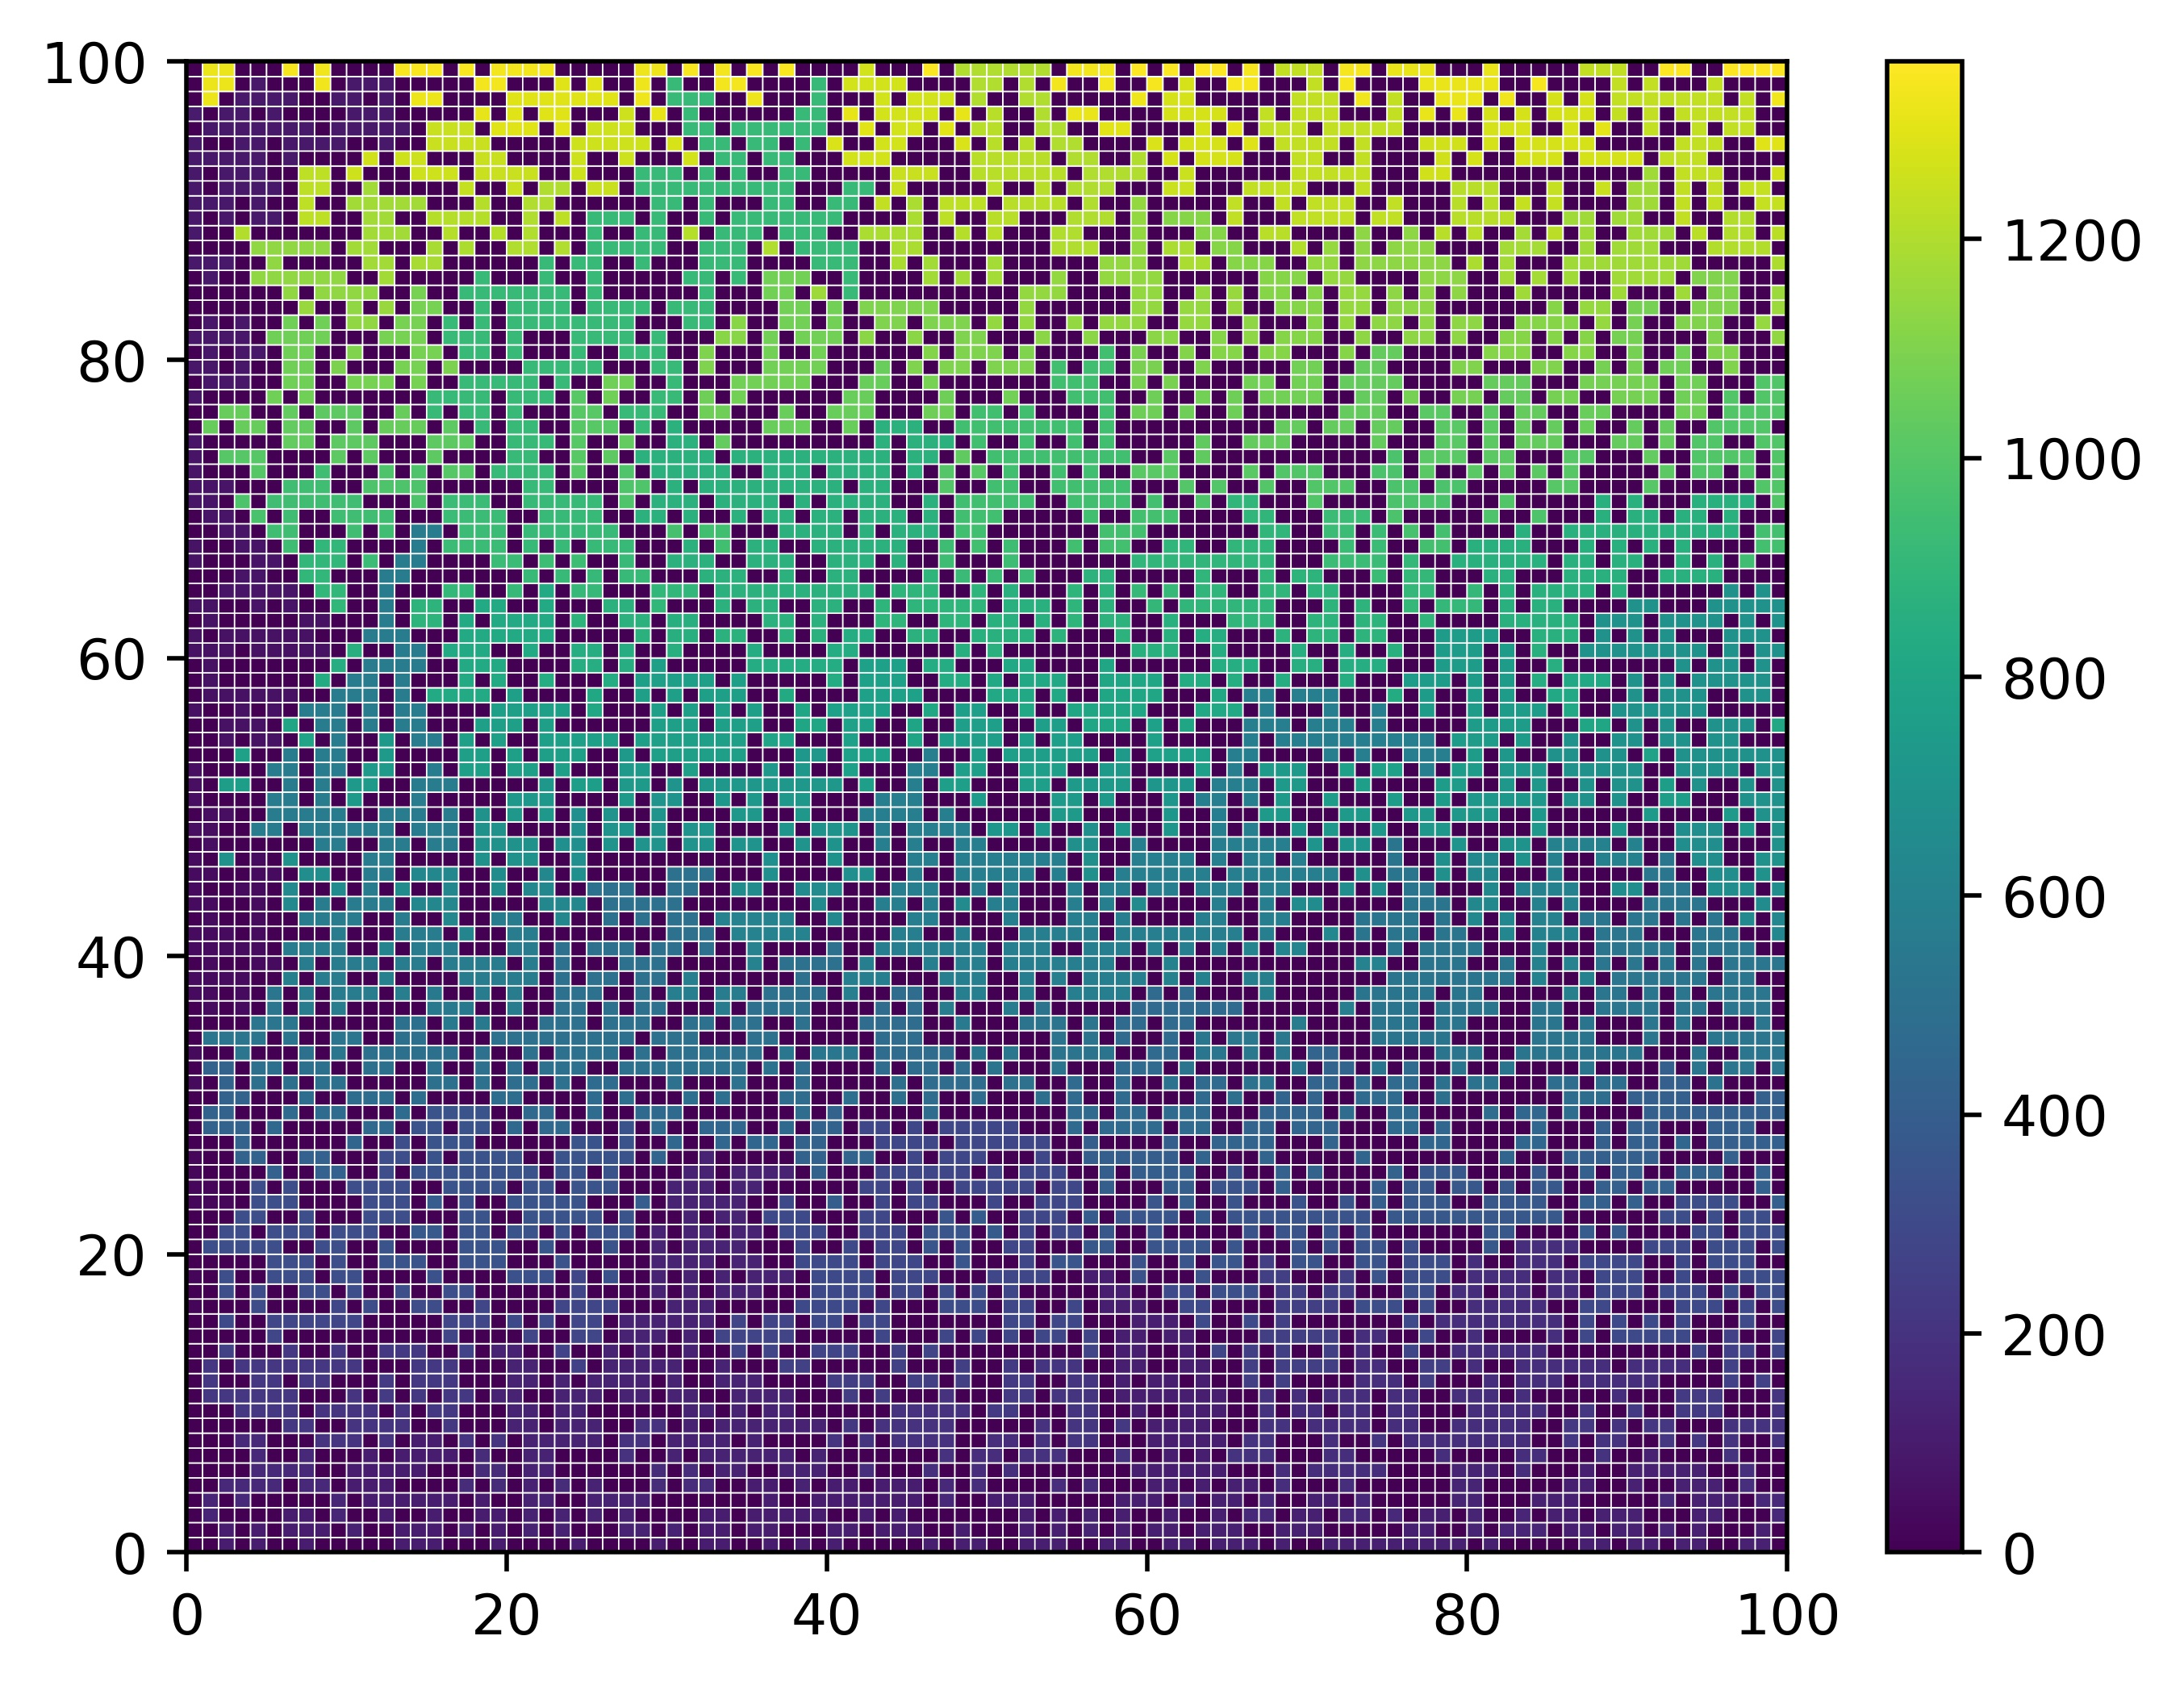
\includegraphics[width=0.9\linewidth]{../p2/colored.jpg}
		\label{fig:Color}
		\caption{Simulation of horizontal percolation for a 100 * 100 grid with probability 0.5. The cells with number 0 are \emph{off} and the ones with the same color form a \emph{clutser}}
	\end{figure}
	
	\section{Probability of Percolation (Question 3)}
	I used the coloring algorithm to find clusters and then a method called \texttt{is\_percolated(grid)} that takes the grid and loops over the last
	column to see if any of the items have a number in the range of the length of our grid. This is the definition of percolation due to the details of
	our clustering and coloring code specified in the previous section.
	I plotted all the data in on plot available in Fig\ref{}.
	
	\section{The Mass Dimention of the Percolation Clusters (Problem 7)}
	I did the simulation 150 times for each probability. I got \texttt{segmentation fault} error for 0.59 so I reduced it to 0.588 and it worked.
	I drew the plots available in Fig\ref{fig:area-gyro}.
	I fitted the data and This is the value to the slope:\\
	\centerline{\texttt{Slope is 1.923 (+/-) 0.009}}
	\begin{figure}[h!]
		\centering
		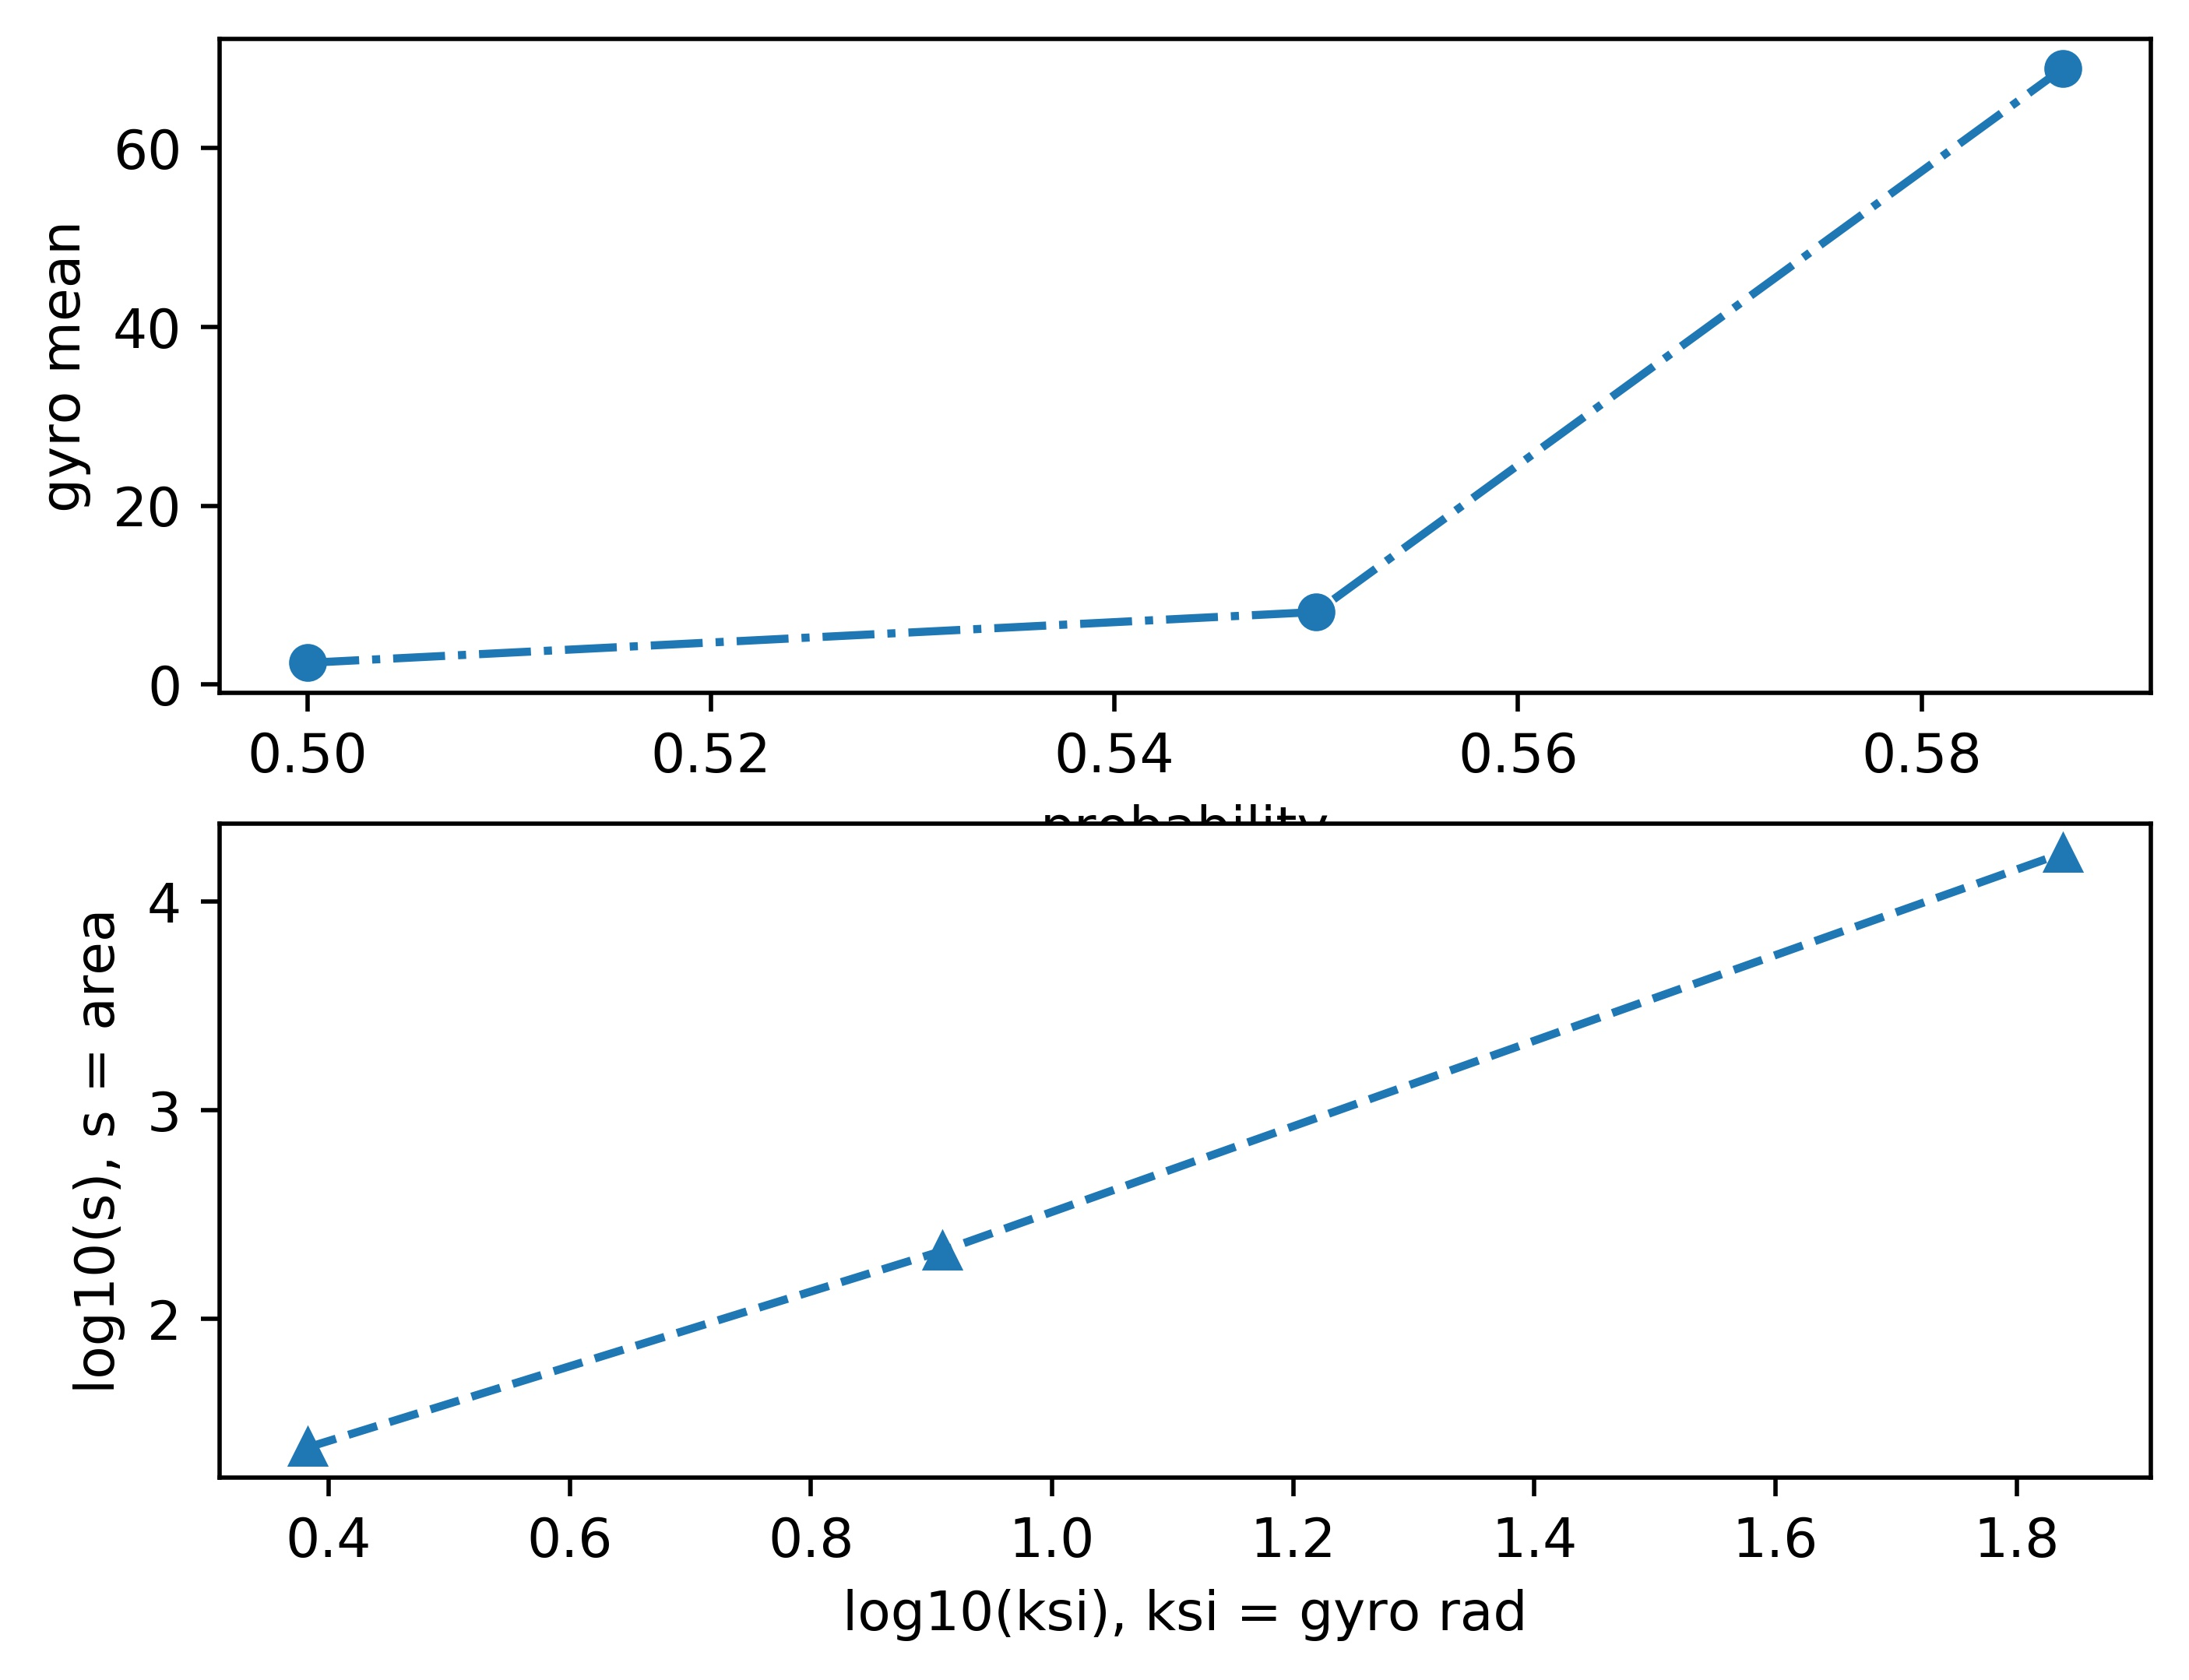
\includegraphics[width=0.9\linewidth]{../p7/area-gyro.jpg}
		\label{fig:area-gyro}
		\caption{I simulated the percolation 150 time for each probability and found reported the mean. Here
		in the top plot you see \emph{gyro radius} vs. \emph{probability}
		and \emph{log of area} vs. \emph{log of gyro radius} in the bottom plot.}
	\end{figure}
\end{document}